%============================================================%
\documentclass[a4paper,12pt]{article}
%%%%%%%%%%%%%%%%%%%%%%%%%%%%%%%%%%%%%%%%%%%%%%%%%%%%%%%%%%%%%%%%%%%%%%%%%%%%%%%%%%%%%%%%%%%%%%%%%%%%%%%%%%%%%%%%%%%%%%%%%%%%%%%%%%%%%%%%%%%%%%%%%%%%%%%%%%%%%%%%%%%%%%%%%%%%%%%%%%%%%%%%%%%%%%%%%%%%%%%%%%%%%%%%%%%%%%%%%%%%%%%%%%%%%%%%%%%%%%%%%%%%%%%%%%%%
\usepackage{eurosym}
\usepackage{vmargin}
\usepackage{amsmath}
\usepackage{graphics}
\usepackage{epsfig}
\usepackage{subfigure}
\usepackage{multicol}
\usepackage{fancyhdr}
\usepackage{listings}
\usepackage{framed}
\usepackage{graphicx}
\usepackage{amsmath}
\usepackage{chngpage}
%\usepackage{bigints}


\setcounter{MaxMatrixCols}{10}

\begin{document}
	\begin{center}
		
\includegraphics[scale=0.55]{images/shieldtransparent2}
	\end{center}
	
	\begin{center}
		\vspace{1cm}
		\large \bf {FACULTY OF SCIENCE AND ENGINEERING} \\[0.5cm]
		\normalsize DEPARTMENT OF MATHEMATICS AND STATISTICS \\[1.25cm]
		\large \bf {END OF SEMESTER EXAMINATION PAPER 2015} \\[1.5cm]
	\end{center}
	
	\begin{tabular}{ll}
		MODULE CODE: MA4505 & SEMESTER: Autumn 2015 \\[1cm]
		MODULE TITLE: Chemometrics & DURATION OF EXAM: 2.5 hours  \\
		 & \\ [1cm]
		LECTURER: Mr. Kevin O'Brien & GRADING SCHEME: 100 marks \\
		& \phantom{GRADING SCHEME:} \footnotesize {70\% of module grade} \\[1cm]
EXTERNAL EXAMINER: Prof. J. King & \\
	\end{tabular}
\vspace{0.3cm}
	\begin{center}
		{\bf INSTRUCTIONS TO CANDIDATES}
	\end{center}
	
	{\noindent \\ Scientific calculators approved by the University of Limerick can be used. \\
		Formula sheet and statistical tables provided at the end of the exam paper.\\
		There are 5 questions in this exam. Students must attempt any 4 questions.}
	%====================================================================== %
	\newpage
\bigskip
%--------------------------------------------------------------------------------------- %

\subsection*{Question 1. (25 marks) Single Sample Inference Procedures and Distributional Testing}\label{sec:question-1.-(25-marks)-inference-procedures-and-distributional-testing}
	
%	\begin{framed}
%		What is going here?
%		\begin{itemize}
%			\item Using the Murdoch Barnes Table for Normal Distribution Problems
%			\item Testing that Data is normally distributed (may appear elsewhere)
%			\item Transformation of Data (Tukey's Ladder)
%			\item Outliers and Boxplots (Grubbs Test, Dixon Q-test)
%			\item Non-Parametric Procedures (e.g. Wilcoxon test, Kolmogorov Smirnov Test)
%		\end{itemize}
%	\end{framed}
%\newpage
%\subsubsection*{Question 1 Part A (4 Marks)}
%%\subsubsection*{Part A Theory for Inference Procedures (4 Marks)}
%Answer the four short questions. Each correct answer will be awarded 1 mark.
%\begin{itemize}
%	\item[(i.)] What is a $p-$value?
%	\item[(ii.)] Briefly describe how $p-$value is used in hypothesis testing.
%	\item[(iii.)] What is meant by a Type I error?
%	\item[(iv.)] What is meant by a Type II error?
%\end{itemize}







\subsubsection*{Question 1 Part A (15 Marks)}
% Clincal 

A test of a specific blood factor has been devised such that, for adults in Western Europe, the test score is normally distributed with mean 100 and standard deviation 10. A clinical research organization is carrying out research on the blood factor levels for sufferers of a particular disease.  

\begin{itemize}
	\item A study has obtained the following test scores for 14 randomly selected patients suffering from the disease in Scotland 
	\[ \{118, 116, 114, 110, 118, 111, 124, 117, 107, 116, 125, 93, 
	106, 119\}\]
	
	\item A similar study has obtained the following test scores for 15 randomly selected patients suffering from the disease in Norway.
	\[\{122, 135, 112, 118, 114, 116, 99, 108, 123, 111, 109, 126, 117, 115, 119\}\]
	
\end{itemize}

% The variance of both data sets are equal. 
% You may assume that both data sets are normally distributed.

%===============================%
% 1. outliers
% 3. variance
% 
%===============================%

\noindent The following blocks of \texttt{R} code (i.e. blocks A to E) are based on the data for this assessment. Write a short report on your conclusion for this assessment. \\ \bigskip

\noindent \textit{\textbf{Marking Scheme}: Either 2 or 3 Marks will be awarded for a correct interpretation of each code segment, for a total of 12 Marks. }

\noindent \textit{State the purpose of each code segment, and then state if it is useful and/or valid in the overall analysis. }

\noindent \textit{Remember to state the null and alternative hypotheses when relevant. 3 Marks will also be award for an overall conclusion. }

\begin{framed}
	\noindent \textbf{Block A} (3 Marks) 
	
	%================================%
	
	\begin{verbatim}
	> grubbs.test(X)
	
	Grubbs test for one outlier
	
	data:  X
	G = 3.11950, U = 0.19387, p-value = 9.184e-05
	..
	
	> grubbs.test(Y)
	
	Grubbs test for one outlier
	
	data:  Y
	G = 2.20890, U = 0.62658, p-value = 0.1164
	
	..
	\end{verbatim}
\end{framed}
%=========================================================================%

\begin{framed}
	\noindent 	\textbf{Block B} (2 Marks)
	\begin{verbatim}
	> shapiro.test(X)
	
	Shapiro-Wilk normality test
	
	data:  X
	W = 0.71132, p-value = 0.0004852
	
	
	> shapiro.test(Y)
	
	Shapiro-Wilk normality test
	
	data:  Y
	W = 0.98139, p-value = 0.9781
	
	\end{verbatim}
\end{framed}
%===========================================================%

\begin{framed}
	\noindent 	\textbf{Block C} (2 Marks)
	\begin{verbatim}
	> var.test(X,Y)
	
	F test to compare two variances
	
	data:  X and Y
	F = 0.65607, num df = 13, denom df = 14, p-value = 0.4544
	alternative hypothesis: true ratio of variances is not equal to 1
	
	95 percent confidence interval:
	0.2178253 2.0219019
	
	sample estimates:
	ratio of variances 
	0.6560667
	
	\end{verbatim}
\end{framed}
%======================================================%
\begin{framed}
	\textbf{Block D}
	\begin{verbatim}
	> wilcox.test(X,Y)
	
	Wilcoxon rank sum test with continuity correction
	
	data:  X and Y
	W = 99, p-value = 0.8098
	alternative hypothesis: true location shift is not equal to 0
	
	
	
	\end{verbatim}	
\end{framed}
\begin{framed}
	\noindent \textbf{Block E} (3 Marks)
	\begin{verbatim}
	> t.test(X,Y,var.equal=TRUE)
	
	Two Sample t-test
	
	data:  X and Y
	t = -0.63849, df = 27, p-value = 0.5285
	alternative hypothesis: true difference in means is not equal to 0
	
	95 percent confidence interval:
	-7.744932  4.068741
	sample estimates:
	mean of x mean of y 
	114.4286  116.2667 
	
	
	> t.test(X,Y,var.equal=FALSE)
	
	Welch Two Sample t-test
	
	data:  X and Y
	t = -0.64325, df = 26.499, p-value = 0.5256
	alternative hypothesis: true difference in means is not equal to 0
	
	95 percent confidence interval:
	-7.706429  4.030238
	sample estimates:
	mean of x mean of y 
	114.4286  116.2667 
	
	\end{verbatim}
\end{framed}
\newpage


%==========================================================%
\subsubsection*{Part A - One Way ANOVA (9 Marks )}
Specimens of milk from dairies in three different districts are assayed for their concentrations of the radioactive isotope Strontium-90. 
The results, in picocuries per litre, are as shown in the table below.

{
	\Large
	\begin{center}
		\begin{tabular}{|c|cccccc|c|c|}
			\hline  
			District & &&&&& & mean & variance \\  
			&  &&&&&& $\bar{x}_i$ & $s^2_{i}$ \\  
			\hline \hline
			A	&	7.6	&	8.1	&	8.5	&	8.3	&	7.9	&	8.8
			&	8.2	&	0.184	\\ \hline
			B	&	8.7	&	10.2	&	11.4	&	10.9	&	7.2	&	9.2
			&	9.6	&	2.404	\\ \hline
			C	&	10.3	&	9.9	&	11.5	&	11.6	&	10.6	&	8.5
			&	10.4	&	1.312	\\ \hline \hline
			Overall & &&&&&&	9.4	&	2.022 \\ \hline	
			
		\end{tabular} 
	\end{center}
}
\bigskip
\begin{itemize}
	\item[(i)] (2 Marks) Showing your workings, compute the \textbf{Between Group Sum of Squares} (\textit{SSbetween}).
	\item[(ii)] (2 Marks) Showing your workings, compute the \textbf{Within Group Sum of Squares}\\ (\textit{SSwithin}).
	\item[(iii)] (2 Mark) Showing your workings, compute the \textbf{Total Group Sum of Squares} (\textit{SStotal}).
	\item[(iv)] (1 Mark) Complete the \textbf{Degrees of Freedom} Column for the ANOVA table below.
	\item[(iv)] (1 Mark) Complete the \textbf{Mean Square} Column for the ANOVA table below.
	\item[(iv)] (1 Mark) Complete the \textbf{F} Column (i.e. the column for Test Statistic) for the ANOVA table below.
\end{itemize}
\bigskip
{
	\Large
	\begin{center}
		\begin{tabular}{|l||c|c|c|c|}
			\hline \phantom{makespace} & DF & SS & MS & F \\ \hline
			\hline Between & \phantom{makespa} &  &  &  \\ 
			\hline Within &  &\phantom{makespace}  &  &  \\ \hline
			\hline Total &  \phantom{makespace} &  &\phantom{makespace}  & \phantom{makespace} \\ 
			\hline 
		\end{tabular} 
	\end{center}
}
%1.	Write out the ANOVA table. You are not required to add the ?Totals? Row. [4 Marks]
%
%2.	Carry out an analysis of variance of these data, conducting your significance test at the 5% level. [2 Marks]

%=================================================================%

\subsubsection*{Part C (5 Marks)}

%\subsubsection*{Part A : Outliers}
\begin{itemize}
	\item[(i.)] (3 Marks) Provide a brief description for three tests from the family of Grubb's  Outliers Tests. Include in your description a statement of the null and alternative hypothesis for each test
	\item[(ii.)] (2 Marks) Describe any required assumptions for tests, and the limitations of these tests.
		\item[(i.)] (3 Marks) Provide a brief description for three tests from the family of Grubbs'  Outliers Tests. Include in your description a statement of the null and alternative hypothesis for each test, any required assumptions and the limitations of these tests.
		\item[(ii.)] (3 Marks) Showing your working, use the Dixon Q Test to test the hypothesis that the lowest value of the following data set is an outlier.
		\[ 11,22,23,24,25,26,29,34\]
\end{itemize}










\newpage
\subsection*{Question 2. (25 marks) Regression Models }
	% Multiple Linear Regression
\subsubsection*{Part A - Short Questions (8 Marks)}	
	\begin{itemize}
		\item[(i)] (1 Mark) In the context of regression models, explain what is meant by Heteroscedascity and Homoescedascity.
		
		
		%-----------------------%
		% Non Parametric 1
		\item[(ii)] (1 Mark)  Explain how the \emph{Akaike information criterion} would used to compare two models fitted for the same data.
		%-----------------------%
		% Non Parametric 2
		\item[(iii)] (1 Mark) Explain why the adjusted $R^2$ value may differ in value from the corresponding multiple $R^2$ value for the same fitted model.
		\item[(iv)] (1 Mark) Write a short note to compare and contrast the multiple R squared and asjusted R squared.
		
	\end{itemize}
	
%=================================================================================%
\subsubsection*{Standard Additions}	
The gold content of a concentrated sea-water sample was determined by using
atomic-absorption spectrometry with the method of standard additions.
\begin{framed}
\begin{verbatim}
> summary(lm(Abso~Gold))

Call:
lm(formula = Abso ~ Gold)

Residuals:
      Min        1Q    Median        3Q       Max 
-0.034662 -0.014833 -0.013924  0.004695  0.096057 

Coefficients:
             Estimate Std. Error t value Pr(>|t|)    
(Intercept) 0.2589060  0.0234791   11.03 4.07e-06 ***
Gold        0.0056720  0.0004668   12.15 1.95e-06 ***
---
Signif. codes:  0 ‘***’ 0.001 ‘**’ 0.01 ‘*’ 0.05 ‘.’ 0.1 ‘ ’ 1

Residual standard error: 0.03852 on 8 degrees of freedom
Multiple R-squared:  0.9486,    Adjusted R-squared:  0.9422 
F-statistic: 147.6 on 1 and 8 DF,  p-value: 1.949e-06

\end{verbatim}
\end{framed}
The results obtained were as follows:


% Gold <-c(30,40,50,60,70,0,10,20,80,70)
% Abso <-c(0.415,0.472,0.528,0.579,0.641,0.271,0.323,0.369,0.678,0.752)

% latex table generated in R 3.3.1 by xtable 1.8-2 package
% Sat Oct 29 21:05:55 2016
\begin{table}[ht]
	\centering
	\begin{tabular}{rrr}
		\hline
Gold Addition   & Absorbance \\
(ng/ml)         & \\

		\hline
		1 & 30.00 & 0.41 \\ 
		2 & 40.00 & 0.47 \\ 
		3 & 50.00 & 0.53 \\ 
		4 & 60.00 & 0.58 \\ 
		5 & 70.00 & 0.64 \\ 
		6 & 0.00 & 0.27 \\ 
		7 & 10.00 & 0.32 \\ 
		8 & 20.00 & 0.37 \\ 
		9 & 80.00 & 0.68 \\ 
		10 & 70.00 & 0.75 \\ 
		\hline
	\end{tabular}
\end{table}


\subsubsection*{Part B - Linear Regression (8 Marks)}
In an experiment to determine hydrolysable tannins in plants by absorption spectroscopy, the following results from ten samples were obtained and are tabulated below. A simple linear regression model, predicting absorbance values using concentration as the independent variable, was fitted to the data. The scatterplot is depicted below.
%%Absorbance= c(0.084, 0.183, 0.326, 0.464, 0.643, 0.707, 0.717, 0.734 ,0.749 ,0.732) ;
%%Concentration= c(0.123, 0.288, 0.562, 0.921, 1.420, 1.717, 1.921, 2.137 ,2.321, 2.467) ;
%%plot(Concentration,Absorbance,pch=18,col="red",font.axis=2,font.lab=2)
%%abline(coef(lm(Absorbance~Concentration)))

%%Conc.Squared = (Concentration^2)
%%Conc.Cubed = (Concentration^3)
%%ModelA = lm(Absorbance~Concentration)
%%ModelB = lm(Absorbance~Concentration+Conc.Squared)
%%ModelC = lm(Absorbance~Concentration+Conc.Squared+Conc.Cubed)
\begin{center}
	\begin{tabular}{|c||c|c|c|c|c|}
		\hline
		%  % after \\: \hline or \cline{col1-col2} \cline{col3-col4} ...
		Sample & 1 & 2 & 3 & 4 & 5 \\ \hline
		Absorbance & 0.084& 0.183& 0.326& 0.464& 0.643\\
		Concentration & 0.123& 0.288& 0.562& 0.921& 1.420\\ \hline
		Sample & 6 & 7 & 8 & 9 & 10 \\ \hline
		Absorbance & 0.707& 0.717& 0.734 &0.749 &0.732\\
		Concentration & 1.717& 1.921& 2.137 &2.321&2.467\\
		\hline
	\end{tabular}
\end{center}
\begin{center}
	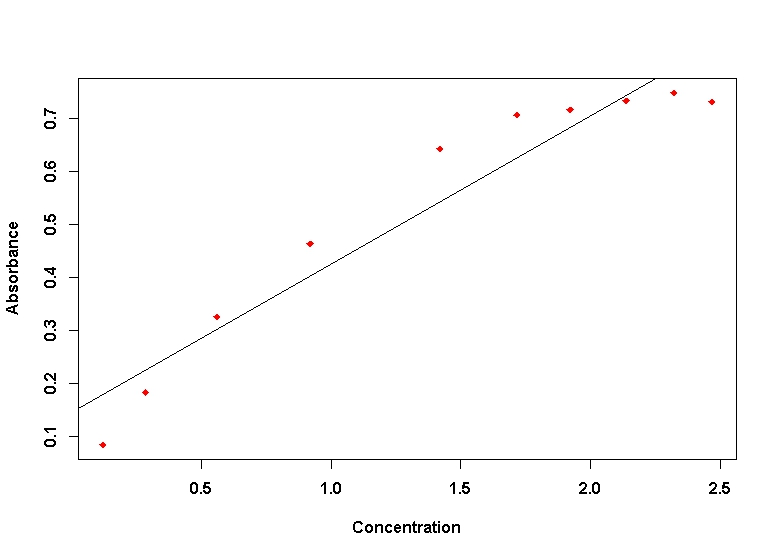
\includegraphics[scale=0.45]{images/ExamQ3plot}
\end{center}
\begin{itemize}
	\item[(i.)] (1 marks) Is the simple linear regression model approach suitable for this study? Explain your answer with reference to the scatter-plot.
	\item[(ii.)] (3 marks) Two polynomial models were also fitted to the data. Description of all three fitted models are found in the three blocks of \texttt{R} code on the following pages. The \emph{Akaike information criterion} is listed, for each of the three fitted models. Write down the regression equations of each of the three models.
	\item[(iii.)] (2 marks) Specify which one of the models you would use. Justify your answer with appropriate statistical values.
	\item[(iv.)] (2 marks) Using the best fitting model, predict a value for absorbance when the concentration level is 1.2 $mg/ml$.
	
\end{itemize}


%
%
%
%\item[(d)] Two polynomial models were also fitted to the data. Description of all three fitted models are found in the three blocks of \texttt{R} code below. The \emph{Akaike information criterion} is also listed, for each of the three fitted models.
%\begin{itemize}
%\item[i.] (4 marks) Write down the regression equation for each of the three linear models.
%\item[ii.] (2 marks) Based on the \emph{Akaike information criterion}, which fitted model can be assumed to be the best fit of the three candidate models.

%\end{itemize}
%\newpage


\begin{framed}
	\noindent \textbf{Model 1}
	\begin{verbatim}
	> summary(Model1)
	Call:
	lm(formula = Absorb ~ Conc)
	...
	Coefficients:
	Estimate Std. Error t value Pr(>|t|)
	(Intercept)    0.14412    0.04721   3.053   0.0158 *
	Concentration  0.28088    0.02930   9.586 1.16e-05 ***
	---
	Signif. codes:  0 ‘***’ 0.001 ‘**’ 0.01 ‘*’ 0.05 ‘.’ 0.1 ‘ ’ 1
	
	Residual standard error: 0.07584 on 8 degrees of freedom
	Multiple R-squared: 0.9199,     Adjusted R-squared: 0.9099
	F-statistic: 91.89 on 1 and 8 DF,  p-value: 1.163e-05
	>
	>
	>AIC(Model1)
	[1] -19.4343
	\end{verbatim}
\end{framed}

\begin{framed}
	\noindent	\textbf{Model 2}
	\begin{verbatim}
	> summary(Model2)
	Call:
	lm(formula = Absorb ~ Conc + Conc.Squared)
	...
	Coefficients:
	Estimate Std. Error t value Pr(>|t|)
	(Intercept)    0.006582   0.008013   0.821    0.439
	Concentration  0.642935   0.015568  41.299 1.27e-09 ***
	Conc.Squared  -0.140573   0.005894 -23.851 5.79e-08 ***
	---
	Signif. codes:  0 ‘***’ 0.001 ‘**’ 0.01 ‘*’ 0.05 ‘.’ 0.1 ‘ ’ 1
	
	Residual standard error: 0.008939 on 7 degrees of freedom
	Multiple R-squared: 0.999,      Adjusted R-squared: 0.9987
	F-statistic:  3592 on 2 and 7 DF,  p-value: 2.879e-11
	>
	>
	> AIC(Model2)
	[1] -61.5338
	\end{verbatim}
\end{framed}


\begin{framed}
	\noindent \textbf{Model 3}
	\begin{verbatim}
	> summary(Model3)
	
	Call:
	lm(formula = Absorb ~ Conc+ Conc.Squared + Conc.Cubed)
	...
	...
	Coefficients:
	Estimate Std. Error t value Pr(>|t|)
	(Intercept)    0.013712   0.011629   1.179   0.2830
	Concentration  0.608682   0.042825  14.213 7.58e-06 ***
	Conc.Squared  -0.108186   0.038088  -2.840   0.0296 *
	Conc.Cubed    -0.008196   0.009518  -0.861   0.4223
	---
	Signif. codes:  0 ‘***’ 0.001 ‘**’ 0.01 ‘*’ 0.05 ‘.’ 0.1 ‘ ’ 1
	
	Residual standard error: 0.009109 on 6 degrees of freedom
	Multiple R-squared: 0.9991,     Adjusted R-squared: 0.9987
	F-statistic:  2306 on 3 and 6 DF,  p-value: 1.422e-09
	>
	>
	> AIC(Model3)
	[1] -60.69903
	\end{verbatim}
\end{framed}
\newpage
%-------------------------------Start of Question 2B%
%\item[(b)](6 marks)
%The scatter-plot contains the regression line for the fitted model. Three diagnostic plots, used to assess the suitability of the fitted model, are presented on the following pages. Provide a brief interpretation for each of the three diagnostic plots described in part(a). The scatter-plot for the data is also presented.

%\begin{center}
%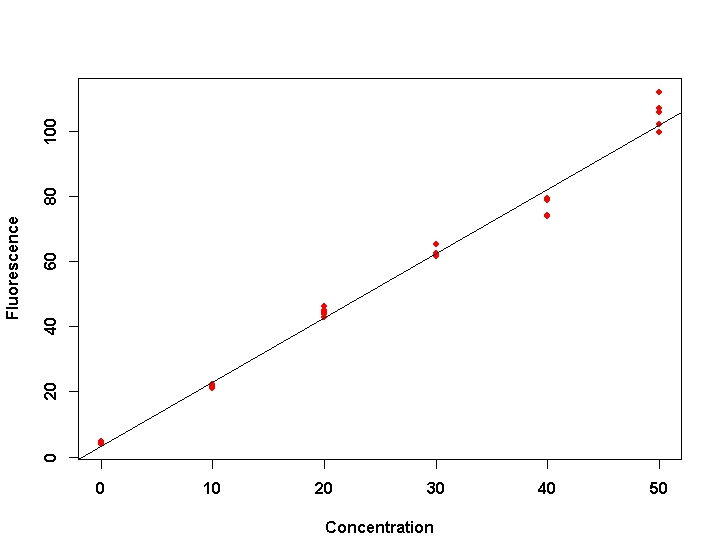
\includegraphics[scale=0.60]{ExamQ2plot2}
%\end{center}
%\newpage
%\begin{center}
%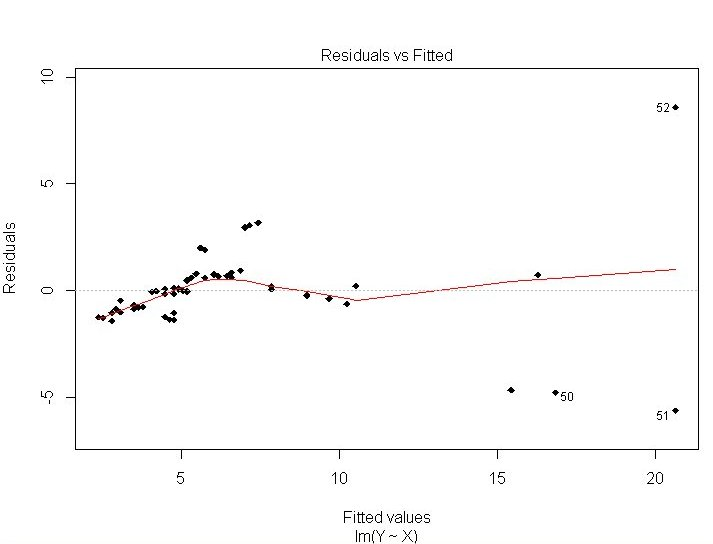
\includegraphics[scale=0.55]{ExamQ2diag1}
%\end{center}
%
%\begin{center}
%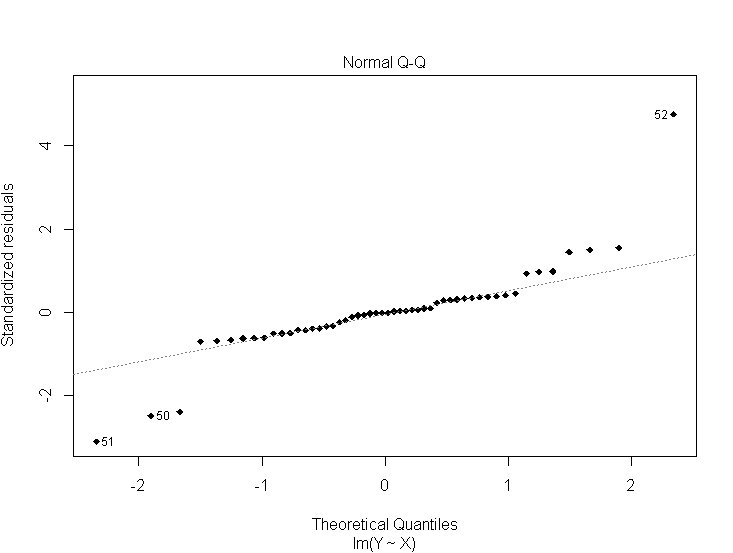
\includegraphics[scale=0.55]{ExamQ2diag2}
%\end{center}
%
%\begin{center}
%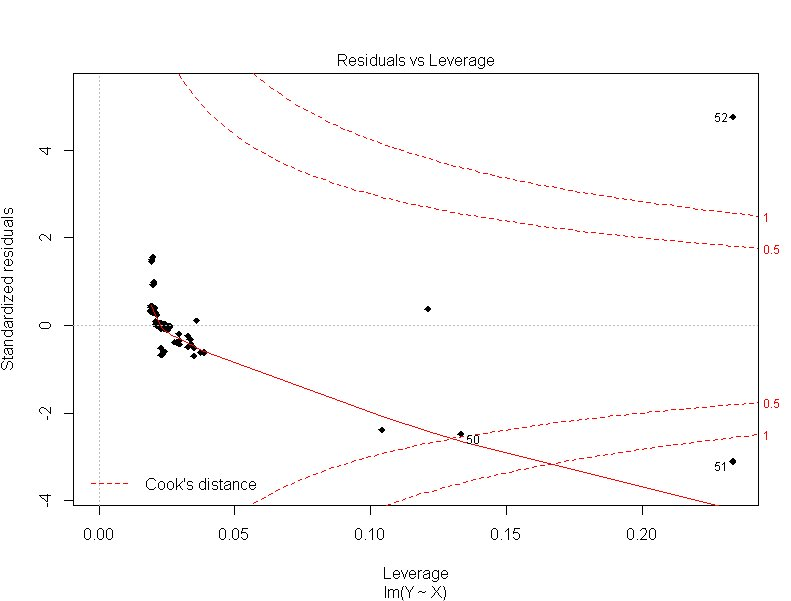
\includegraphics[scale=0.55]{ExamQ2diag3}
%\end{center}

%%-------------------------------End  of Question 2B%
%\newpage
%\subsubsection*{Question 2 Part B (10 Marks)}	
% Complete the following \textit{Analysis of Variance} Table for a simple linear regression model based on the data provided. The required values are indicated by question marks.
%\begin{center}
%	\begin{tabular}{|c|c|c|c|c|c|} \hline
%		& Df & 	Sum Sq &	Mean Sq &	F value &   	Pr($>$F)    \\ \hline
%		Regression &  ? &	9160239 &	? &	 ? &	$< 2.2e^{-16}$ \\ \hline
%		Error  & 50 &	2134710 &  	?   &            &       \\ \hline
%		Total  & ?  &	? &  	42694   &            &       \\ \hline
%	\end{tabular} 
%\end{center}
%
%Once you have completed this table, compute the following
%\begin{itemize}
%	\item (1 Mark) The Pearson correlation coefficient for the response variable Y and the predictor variable X.
%	\item (1 Mark) The sample standard deviation of the response variable Y.
%\end{itemize}


\subsubsection*{Part C - Robust Regression (7 Marks)}

% \subsection*{Q9.Robust Regression}
%Write a brief explanation of how robust regression differs from linear models computed using the \emph{Ordinary Least Squares method}, making reference to one particular weighting method only. Provide a description on how this weighting method works.


In certain circumstances, Robust Regression may be used in preference to Ordinary Least Squares Regression. Answer the following questions relating to Robust Regression. 

\begin{itemize}
	\item[(i.)] (1 Mark) Describe what these circumstances might be.
	\item[(ii.)] (1 Mark) State one difference between OLS and Robust regression techniques, in terms of computing regression equations.
	\item[(iii.)] (2 Marks) Explain the process of Huber Weighting for Residuals, stating the algorithm used to compute weightings.
	\item[(iv.)] (3 Marks) Suppose that Huber Weighting, with a tuning constanct of $k=13.45$, was applied to the observations 
	tabulated below. What would be the outcome of the procedure for each case. 
\end{itemize}
\begin{center}
	\begin{tabular}{|c|c|}
		\hline
		Observation & Residual \\ 
		$i$  & $e_i$ \\ \hline
		11 & -9.07 \\ \hline 
		14 & 14.54 \\ \hline
		18 & 22.91 \\ \hline
	\end{tabular} 
\end{center}

\subsubsection*{ Part C Influence (10 Marks)}
%The following scatterplot
%\begin{figure}[h!]
%\centering
%\includegraphics[width=0.8\linewidth]{images/ExamQ2diagnostics}
%\end{figure}
\begin{itemize}
	\item[(i.)] (1 Marks) Explain the term ``Influence" in the context of linear regression models. Support your answer with sketches.
	\item[(ii.)] (1 Marks) Explain the  term ``Cook's Distance" in the context of linear regression models. 
	\item[(iii.)] (2 Marks) The following plot is the \textit{Residual vs Fitted} plot, the first of \texttt{R}'s diagnostic plots for linear models. Briefly describe how to interpet this plot. What is your conclusion?
%%	\begin{figure}[h!]
%%		\centering
%%		\includegraphics[width=0.8\linewidth]{images/ExamQ2diag1anscombe}
%%	\end{figure}
	\newpage
	\item[(iv.)] (2 Marks) Explain the term ``Heteroscedascity" in the context of linear regression models. Support your answer with sketches.
	\item[(v.)] (1 Mark) The Outliers Test Test was carried out to test for Heteroscedascity. The output is depicted below. State your conclusion to the following procedure.
	
	%\begin{framed}
	%	\begin{verbatim}
	%	> ncvTest(ModelQ2)
	%	Non-constant Variance Score Test 
	%	Variance formula: ~ fitted.values 
	%	Chisquare = 7.585432    Df = 1     p = 0.005884187
	%	\end{verbatim}
	%\end{framed}
	%
	%\item[(vi)] (3 Marks) Outliers Test
	\begin{framed}
		\begin{verbatim}
		> outlierTest(ModelQ2)
		rstudent unadjusted p-value Bonferonni p
		3 1203.539         2.5441e-22   2.7985e-21
		\end{verbatim}
	\end{framed}
	
	\item[(vi.)] (2 Marks)  The Durbin Watson Test was carried out to test for Autocorrelation. Briefly describe autocorrelation. You may support your answer with sketches.
	\item[(vii.)] (1 Mark) State your conclusion to the following procedure.
	\begin{framed}
		\begin{verbatim}
		> durbinWatsonTest(ModelQ2)
		lag Autocorrelation D-W Statistic p-value
		1     -0.08428163      2.143578   0.806
		Alternative hypothesis: rho != 0
		\end{verbatim}
	\end{framed}
	
\end{itemize}








%%-------------------------------------%
%\subsection*{Question 3. (20 marks) Multiple Linear Regression Models }
%\begin{itemize}
%
%\item[(a)] Explain the following terms:
%\begin{itemize}
%\item[i.] (2 marks) Over-fitting,
%\item[ii.] (2 marks) Multicollinearity,

%\end{itemize}
%\item[(b)] Answer the following questions related to model selection techniques for linear models.
%\begin{itemize}
%\item[i.] (2 marks) Explain why the adjusted $R^2$ value may differ in value from the corresponding multiple $R^2$ value for the same fitted model.
%\item[ii.] (2 marks) Explain how the \emph{Akaike information criterion} would used to compare two models fitted for the same data.
%\end{itemize}
%


\subsubsection*{Question 3 Part D (12 Marks)}
The mercury level of several tests of sea-water from costal areas was determined by atomic-absorption spectrometry. The results obtained are as follows
\begin{center}
	\begin{tabular}{|c||c|c|c|c|c|c|c|c|c|c|c|} \hline
		Conc &0 &10&20&30&40&50&60&70&80&90&100 \\ \hline 
		Abso &0.321& 0.834& 1.254& 1.773& 2.237& 2.741& 3.196& 3.678& 
		4.217& 4.774& 5.261 \\ \hline
	\end{tabular} 
	
\end{center}


The analysis of the relationship between concentration and absorbance is obtained in R and presented below. 
\begin{framed}
	\begin{verbatim}
	x<-seq(0,100,by=10)
	y<- c(0.321, 0.834, 1.254, 1.773, 2.237, 2.741, 3.196, 3.678, 
	4.217, 4.774, 5.261)
	model<- lm(y~x)
	summary(model)
	
	Call:
	lm(formula = y ~ x)
	
	Coefficients:
	Estimate Std. Error t value Pr(>|t|)    
	(Intercept) 0.2933636  0.0234754   12.50 5.45e-07 
	x           0.0491982  0.0003968  123.98 7.34e-16 
	---
	
	Residual standard error: 0.04162 on 9 degrees of freedom
	Multiple R-squared: 0.9994,     Adjusted R-squared: 0.9993 
	F-statistic: 1.537e+04 on 1 and 9 DF,  p-value: 7.337e-16 
	
	confint(model)
	                 2.5 %     97.5 %
	(Intercept) 0.24025851 0.34646876
	x           0.04830054 0.05009582
	
	\end{verbatim}
\end{framed}

\begin{itemize}
	\item[(i)] (2 marks)
	Determine and interpret the slope and the intercept of the regression line.
	\item[(ii)]  (2 marks) State the 95\% confidence interval for the slope and the intercept coefficients. Interpret this intervals with respect to any relevant hypothesis tests
	\item[(iii)] (2 marks) Explain in which way is the prediction intervals different from the confidence intervals for fitted values in linear regression?
	\item[(iv)] (2 Marks) The following piece of \texttt{R} code gives us a statistical metric. What is this metric? What is it used for? How should it be interpreted.
	
\end{itemize}
\begin{framed}
	\begin{verbatim}
	> AIC(model)
	[1] -34.93389	
	\end{verbatim}
\end{framed}

%=====================================================



%================================================= %

\subsubsection*{Part B Regression ANOVA (6 Marks)}
Suppose we have a regression model, described by the following equation
\[ \hat{y} = 28.81 + 6.45x_1 + 7.82 x_2\]
We are given the following pieces of information.
\begin{itemize}
	\item The standard deviation of the response variance $y$ is 10 units.
	\item There are 53 observations.
	\item The \textit{Coefficient of Determination} (also known as the \textit{Multiple R-Squared}) is 0.75.
\end{itemize}
Complete the \textit{Analysis of Variance} Table for a linear regression model.
The required values are indicated by question marks.

\begin{center}
	\begin{tabular}{|c|c|c|c|c|c|} \hline
		\phantom{makespace}	& DF & 	Sum Sq &	Mean Sq &	F value &   	Pr($>$F)    \\ \hline
		Regression &  \phantom{make}?\phantom{make} &	? &	? &	 ? &	$< 2.2e^{-16}$ \\ \hline
		Error  & ? &	? &  	?   &            &       \\ \hline
		Total  & ?  &	? &  \phantom{makespace}	  &   \phantom{makespace}         &    \phantom{makespace}    \\ \hline
	\end{tabular} 
\end{center}



%======================================================
\subsection*{Question 3. (25 marks) Experimental Design }


\subsubsection*{Question 2 - Two Way ANOVA (6 Marks )}

\begin{enumerate}[(i)]
%-----------------------%
	\item (4 marks) What is the purpose of a post hoc test?
	\item (4 marks) What are the key components that need to be identified when designing an
experiment?
	\item (4 marks) What is a completely randomised design?
	\item (4 marks) What is a randomised block design?

\item (4 marks) What is an ``$a \times b$" factorial experimental design?
	\item (4 marks)  What is the difference between a between-treatments estimate and a withintreatments
estimate?
	\item (4 marks) What distinguishes a factorial experiment from a completely randomised experiment or a randomised block experiment?
\end{enumerate}}	





\subsubsection*{Question 2 - Two Way ANOVA (6 Marks )}
\noindent Suppose you want to determine whether the brand of cleaning product used and the temperature affects the amount of dirt removed from your machinery. 

\noindent You are also interested in determining if there is an interaction between the two variables.


\noindent You buy two different brand of detergent (``\textit{Super}" and ``\textit{Best}") and choose three different temperature levels (``\textit{Cold}?, ``\textit{Warm}", and ``\textit{Hot}"). There are four measurements per treatment group.
{
	\large
	\begin{center}
		\begin{tabular}{|c||c|c|c|}
			\hline
			& Cold & Warm & Hot  \\ \hline \hline
			Super &  4,5,6,5    & 7,9,8,12     &  10,12,11,9    \\  \hline
			Best  &  6,6,4,4    & 13,15,12,12    & 12,13,10,13     \\  \hline
		\end{tabular} 
	\end{center}
}
\begin{itemize}
	\item Detergent is Factor A.
	\item Temperature is Factor B.
	\item The variance of the response variable is 12.2011.
\end{itemize}
%---------------------------------------------------%
{
	\large
	\begin{center}
		\begin{tabular}{|c|c|c|c|c|}\hline
			Source & DF & SS & MS & F \\ \hline
			A  & \phantom{spa}? \phantom{spa}  & 22.04 & \phantom{spa}? \phantom{spa} & \phantom{spa}? \phantom{spa} \\ \hline
			B  &\phantom{spa}? \phantom{spa} & \phantom{spa}? \phantom{spa}  & 102.37 & \phantom{spa}? \phantom{spa} \\ \hline
			A:B  & \phantom{spa}? \phantom{spa}& 16.08 & \phantom{spa}? \phantom{spa} & \phantom{spa}? \phantom{spa} \\ \hline
			Resid & \phantom{spa}? \phantom{spa}& \phantom{spa}? \phantom{spa} & \phantom{spa}? \phantom{spa} & \\ \hline \hline
			Total & \phantom{spa}? \phantom{spa}&\phantom{spa}? \phantom{spa}  & \phantom{spa} & \\  \hline
		\end{tabular} 
	\end{center}
}

\subsubsection*{Water Nitrate (One Way ANOVA MA4605)}
	Four investigators, A, B, C and D, performed six determination of nitrate in water using the same procedure. The results in $\mu$M were:
	
	% Investigator 1 Investigator 2 Investigator 3
	
	\begin{center}
		\begin{tabular}{|c|c|c|c|} \hline
			A  &  B   & C &D\\ \hline \hline
			6.7 & 6.3 & 6.8 & 6.9\\ \hline
			6.8 & 6.2 & 6.9 & 7.1\\ \hline
			6.5 & 6.1 & 7.1 &6.3 \\ \hline
			6.8 & 6.3 & 6.9 &6.2\\ \hline
			6.9 & 6.5 & 7.2 & 6.1\\ \hline
			7.1 & 6.4 & 7.1 & 6.4\\ \hline
		\end{tabular} 
	\end{center}
	
	
	
	\noindent We are also given the summmary statistics for each of the three investigators, as well as for the samples combined.
	\begin{center}
		\begin{tabular}{|c|c|c|}
			\hline  & Sample Mean & Sample Variance \\ 
			\hline A & 6.8 & 0.040 \\ 
			\hline B & 6.3 & 0.020 \\ 
			\hline C & 7 & 0.024 \\ 
			\hline D & 6.5 &  0.164\\
			\hline Overall & 6.65 & 0.1295 \\ 
			\hline 
		\end{tabular} 
	\end{center}
	\noindent An analysis of variance procedure is used to determine if there is a significant difference between the mean of the determinations made by the three investigators.
	
	% The following output is obtained in R and presented below.
	
	%investigator <- c(6.7, 6.8, 6.5, 6.8, 6.9, 7.1, 6.3, 6.2, 6.1, 6.3, 6.5, 6.4, 
	%6.8, 6.9, 7.1, 6.9, 7.2, 7.1)
	%A <- investigator[1:6]
	%B <- investigator[7:12]
	%C <- investigator[13:18]
	%
	%
	%
	%group <- factor(rep(1:3,each=6))
	%
	%aov(investigator~group)
	%
	%Analysis of Variance Table
	%
	%Response: investigator
	
	%Df SumSq MeanSq Fvalue Pr(>F)
	%
	%group ? 1.42333 ? ? 3.133e-05
	%
	%Residuals 15 ? ?
	%
	%Total ? 1.9
	\smallskip
	
	\noindent The following questions will result in the completion of the ANOVA Table on the next page. The $p-$value is already provided.
	\begin{itemize}
		\item[(i.)](3 Marks) Compute the Between Groups Sum of Squares. (Show your workings.)
		\item[(ii.)](3 Marks) Compute the Within Groups Sum of Squares.(Show your workings.)
		\item[(iii.)](2 Marks) Compute the Total Sum of Squares. (Show your workings).
		\item[(iv.)] (1 Mark) State the degrees of freedom for the ANOVA Tables
		\item[(v.)] (1 Mark) Compute the Mean Square values.
		\item[(vi.)] (1 Marks) Compute the test Statistic for this procedure (i.e. the F-value.)
		\item[(vii.)] (3 Marks) This analysis is used to assess if there is any difference between the mean determinations made by the three investigators. What is your conclusion? Clearly state the null and alternative hypothesis.
	\end{itemize}
	%================================================================================ %
	\begin{center}
		\begin{tabular}{|c||c|c|c|c|c|}
			\hline Source & DF & SS & MS & F & p-value \\ \hline 
			\hline Between & \phantom{mak} ? \phantom{mak}  & \phantom{mak} ? \phantom{mak}  & \phantom{mak} ? \phantom{mak}  & \phantom{mak} ? \phantom{mak}  &  $0.000454$ \\ 
			\hline Within &  ? & ? & \phantom{mak} ? \phantom{mak}  &  &  \\ 
			\hline \hline Total & ? & ? &  &  &  \\ 
			\hline 
		\end{tabular}
	\end{center} 
	%===================================================================================================== %

	%\subsubsection*{Question 4 Part B (10 Marks)}
	%
	%
	%
	%
	%The \texttt{R} code and graphical procedures, below and on the following page, are relevant to checking whether the underlying assumptions are met for the ANOVA model in part (b).
	%\begin{itemize}
	%	\item[i.] (3 marks) What are the assumptions underlying ANOVA?
	%	\item[ii.] (4 marks)  Assess the validity of these assumptions for the ANOVA model in part(b).
	%	
	%\end{itemize}
	%\begin{framed}
	%	\begin{verbatim}
	%	Shapiro-Wilk normality test
	%	
	%	data:  Residuals
	%	W = 0.9719, p-value = 0.3819
	%	\end{verbatim}
	%\end{framed}
	%\begin{framed}
	%	\begin{verbatim}
	%	Bartlett test of homogeneity of variances
	%	
	%	data:  Experiment
	%	Bartlett's K-squared = 105.9585, df = 1, p-value < 2.2e-16
	%	\end{verbatim}
	%\end{framed}
	%\begin{center}
	%	\includegraphics[scale=0.59]{images/ExamQ5boxplot}
	%\end{center}
	%\newpage
	%%qqnorm(resid(Model),pch=18,col="red",font.lab=2,font.axis=2)
	%%qqline(resid(Model))
	%\begin{center}
	%	\includegraphics[scale=0.55]{images/ExamQ5qqplot}
	%\end{center}
	%\begin{center}
	%	\includegraphics[scale=0.55]{images/ExamQ5resid}
	%\end{center}
	%-----------------------------------------------------------------%
	
	% End of Question
	\newpage
	\normalsize{

		\subsubsection*{Question 3 Part B (4 Marks) - check ANOVA Assumptions}
		The \texttt{R} code and graphical procedures, below and on the following page, are relevant to checking whether the underlying assumptions are met for an ANOVA model.
		\begin{itemize}
			\item[(i.)] (2 marks) State two testable assumptions required for ANOVA procedures? (You may refer to the code output below.)
			\item[(ii.)] (2 marks)  Assess the validity of these assumptions for an ANOVA model based on the following code outputs.
			
		\end{itemize}
		{
			\normalsize
			\begin{framed}
				\begin{verbatim}
				> #Shapiro-Wilk normality test
				> shapiro.test(resid(model))
				
				Shapiro-Wilk normality test
				
				data:  resid(model)
				W = 0.96108, p-value = 0.4604
				
				\end{verbatim}
			\end{framed}
			\begin{framed}
				\begin{verbatim}
				> bartlett.test(investigator~group)
				
				Bartlett test of homogeneity of variances
				
				data:  investigator by group
				Bartlett's K-squared = 7.1354, df = 3, p-value = 0.0677
				
				\end{verbatim}
			\end{framed}
		}
		% \begin{center}
		% 	\includegraphics[scale=0.59]{image/ExamQ5boxplot}
		% \end{center}
		% \newpage
		% %qqnorm(resid(Model),pch=18,col="red",font.lab=2,font.axis=2)
		% %qqline(resid(Model))
		% \begin{center}
		% 	\includegraphics[scale=0.55]{image/ExamQ5qqplot}
		% \end{center}
		% \begin{center}
		% 	\includegraphics[scale=0.55]{image/ExamQ5resid}
		% \end{center}
	}
	\newpage
	
	\subsubsection*{Question 3 Part C (7 Marks) Two Way ANOVA No Replicates}
	\noindent A supermarket buys a particular product from five suppliers (V,W,X,Y and Z), and conducts regular tasting tests by three expert panels.
	%are carried out as the product is sold in their food halls. 
	Various characteristics are scored and an analysis of the totals of these scores is made. 
	
	\begin{center}
		\begin{tabular}{|c|c|c|c|c|c|}\hline 
			&	V  & W  & X & Y & Z \\ \hline
			\hline  
			
			Panel 1&   22 &  25 &  23 &  23 &  24 \\ \hline
			Panel 2&   21 &  16 &  16 &  19 &  16 \\ \hline
			Panel 3&   23 &  22 &  19 &  23 &  22 \\ \hline
			
			\hline 
		\end{tabular} 
	\end{center}
	
	\noindent You are also given the following information:
	\begin{itemize}
		\item $S^2_r = 8.9733$
		\item $S^2_c = 1.0777$
		\item The variance of scores in the table above is $\mbox{Var}(y) = 9.0666$
	\end{itemize}
	\bigskip 
	\noindent The following questions will result in the completion of the ANOVA Table on the bottom of this page. The $p-$values for both tests are already provided.
	\begin{itemize}
		\item[(i.)](4 Marks) Complete the Sum of Squares column. (Show your workings.)
		\item[(ii.)] (1 Mark) State the degrees of freedom for the ANOVA Table.
		%		\item[(v.)] (1 Marks) Compute the Mean Square values.
		%		\item[(vi.)] (1 Mark) Compute the test statistics for this procedure (i.e. the F-values).
		\item[(iii.)] (2 Marks) Based on the p-values, provided, what is your conclusion? Clearly state the null and alternative hypotheses for both tests.
	\end{itemize}
	
	\begin{center}
		\begin{tabular}{|c||c|c|c|c|l|}
			\hline Source & DF & SS & MS & F & p-value \\ \hline 
			\hline Factor A & \phantom{mak} ? \phantom{mak}  & \phantom{mak} ? \phantom{mak}  & \phantom{mak} ? \phantom{mak}  & \phantom{mak} ? \phantom{mak}  &0.00205 ** \\ \hline
			\hline Factor B & \phantom{mak} ? \phantom{mak}  & \phantom{mak} ? \phantom{mak}  & \phantom{mak} ? \phantom{mak}  & \phantom{mak} ? \phantom{mak}  & 0.43290    \\ \hline
			\hline Error &  ? & ? & \phantom{mak} ? \phantom{mak}  &  &  \\ 
			\hline \hline Total & ? & ? &  &  &  \\ 
			\hline 
		\end{tabular}
	\end{center} 
	
	
	
	
	
	
	
	
	
	
	

\subsubsection*{One-Way ANOVA F-test}




	\section*{Question 2 - Two Way ANOVA with Replicates(6 Marks )}
	\noindent Suppose you want to determine whether the brand of cleaning product used and the temperature affects the amount of dirt removed from your machinery. 
	
	\noindent You are also interested in determining if there is an interaction between the two variables.
	
	
	\noindent You buy two different brand of detergent (``\textit{Super}" and ``\textit{Best}") and choose three different temperature levels (``\textit{Cold}”, ``\textit{Warm}", and ``\textit{Hot}"). There are four measurements per treatment group.
	{
		\Large
		\begin{center}
			\begin{tabular}{|c||c|c|c|}
				\hline
				& Cold & Warm & Hot  \\ \hline \hline
				Super &  4,5,6,5    & 7,9,8,12     &  10,12,11,9    \\  \hline
				Best  &  6,6,4,4    & 13,15,12,12    & 12,13,10,13     \\  \hline
			\end{tabular} 
		\end{center}
	}
	\begin{itemize}
		\item Detergent is Factor A.
		\item Temperature is Factor B.
		\item The variance of the response variable is 12.2011.
	\end{itemize}
\noindent \textbf{Exercises}
For the Table above, replace the questions marks with the correct values in each of the following columns. (The number of marks for each column is indicated here:)
\begin{itemize}
	\item[(i)] (2 Marks) Degrees of freedom 
	\item[(ii)](2 Mark) Sums of Squares column
	\item[(iii)](1 Mark) Mean Square Values
	\item[(iv)](1 Mark)F-Values
\end{itemize}


{
	\large
	\begin{center}
		\begin{center}
			\begin{tabular}{|c|c|c|c|c|}\hline
				Source & DF & SS & MS & F \\ \hline
				A  & \phantom{makespace}  & \phantom{makespace} & \phantom{makespace} & \phantom{makespace} \\ \hline
				B  &\phantom{makespace} & \phantom{makespace}  & \phantom{makespace}& \phantom{makespace} \\ \hline
				A:B  & \phantom{makespace}& \phantom{makespace} & \phantom{makespace} & \phantom{makespace} \\ \hline
				Resid & \phantom{makespace}& \phantom{makespace} & \phantom{makespace} & \\ \hline \hline
				Total & \phantom{makespace}&\phantom{makespace}  & \phantom{spa} & \\  \hline
			\end{tabular} 
		\end{center}
	\end{center}
}


\subsubsection*{Question 3 Part C (7 Marks)}
Six analysts each made seven determinations of the paracetamol content of the same batch of tablets.
The results are shown below. There are 42 determinations in total. 
%The mean determination for each analysts is also tabulated. \\


%Analyst= structure(c(1L, 2L, 3L, 4L, 5L, 6L, 1L, 2L, 3L, 4L, 5L, 6L, 1L,
%2L, 3L, 4L, 5L, 6L, 1L, 2L, 3L, 4L, 5L, 6L, 1L, 2L, 3L, 4L, 5L,
%6L, 1L, 2L, 3L, 4L, 5L, 6L, 1L, 2L, 3L, 4L, 5L, 6L), .Label = c("A",
%"B", "C", "D", "E", "F"), class = "factor")

%Determinations= c(84.32, 84.24, 84.29, 84.14, 84.5, 84.7, 84.61, 84.13, 84.28,
%84.48, 83.91, 84.36, 84.64, 84, 84.4, 84.27, 84.11, 84.61, 84.62,
%84.02, 84.63, 84.22, 83.99, 84.15, 84.51, 84.25, 84.4, 84.22,
%83.88, 84.17, 84.63, 84.41, 84.68, 84.02, 84.49, 84.11, 84.51,
%84.3, 84.36, 84.33, 84.06, 83.81)

\begin{center}
	\begin{tabular}{|c|ccccccc|}
		\hline
		Analyst	& Content		&		&		&		&		&		&		 \\ \hline
		A	&	84.32	&	84.61	&	84.64	&	84.62	&	84.51	&	84.63	&	84.51	 \\
		B	&	84.24	&	84.13	&	84.00	&	84.02	&	84.25	&	84.41	&	84.30	 \\
		C	&	84.29	&	84.28	&	84.40	&	84.63	&	84.40	&	84.68	&	84.36	 \\
		D	&	84.14	&	84.48	&	84.27	&	84.22	&	84.22	&	84.02	&	84.33	 \\
		E	&	84.50	&	83.91	&	84.11	&	83.99	&	83.88	&	84.49	&	84.06	 \\
		F	&	84.70	&	84.36	&	84.61	&	84.15	&	84.17	&	84.11	&	83.81	 \\
		\hline
	\end{tabular}
\end{center}
\bigskip
The following \texttt{R} output has been produced as a result of analysis of these data:

%Experiment=data.frame(Determinations, Analyst)
%Model=aov(Determinations~Analyst)
%summary(Model)
\begin{framed}
	\begin{verbatim}
	Analysis of Variance Table
	
	Df   Sum Sq   Mean Sq   F value    Pr(>F)
	Analyst        5   0.8611   0.17222     4.236   0.00394 **
	Residuals     36   1.4635   0.04065
	---
	Signif. codes:  0 ‘***’ 0.001 ‘**’ 0.01 ‘*’ 0.05 ‘.’ 0.1 ‘ ’ 1
	\end{verbatim}
\end{framed}

%\subsubsection*{Vegetables (ONE WAY ANOVA 4505)}
%
%(c) The following data give the recovery of bromide from spiked samples of vegetable matter, measured using a gas-liquid chromatographic method. The same amount of bromide was added to each specimen. 
%
%The units for all measurements are  mg g-1
%
%\begin{center}
%	\begin{tabular}{|c|c|c|c|}
%		Tomato: & $\{777 790 759 790 770 758 764\}$ & 774 & 142.6667
%		\\ \hline
%		
%		Cucumber: & $\{782 773 778 765 789 797 782\}$ & 781 &  106\\ \hline
%		
%		Asparagus : & $\{786 783 781 785 789 797 782 \}$& 785 & \\ \hline
%	\end{tabular} 
%\end{center}


%-------------------------------------------------------------------------------
%y<-c(777, 789, 769, 790, 770, 759, 764, 782, 774, 778, 765, 789, 
%797, 782, 785, 783, 782, 785, 787, 791, 782)
%
%
%
%T<-y[1:7];C<-y[8:14];A<-y[15:21];
%mean(T);mean(C);mean(A);
%
%-------------------------------------------------------------------------------
%-------------------------------------------------------------------------------

%
%
%\begin{itemize}
%	\item[(i)](3 Marks) Compute the Between Groups Sum of Squares, \textit{Show your workings}
%	\item[(ii)](3 Marks) Compute the Within Groups Sum of Squares, \textit{Show your workings}
%	\item[(iii)](2 Marks) Compute the Total Sum of Squares,\textit{ show your workings}
%	\item[(iv)] (2 Marks) Degrees of Fredom columns
%	\item[(v)] (1 Marks) Mean Square
%	\item[(vi)] (1 Marks) F test Statistics
%\end{itemize}
%\begin{tabular}{|c|c|c|c|c|c|}
%	\hline Source & DF & SS & MS & F & p-value \\ 
%	\hline Between &  &  &  &  &  \\ 
%	\hline Within &  &  &  &  &  \\ 
%	\hline Total &  &  &  &  &  \\ 
%	\hline 
%\end{tabular} 
%\begin{framed}
%	\begin{verbatim}
%	> bartlett.test(y~group)
%	
%	Bartlett test of homogeneity of variances
%	
%	data:  y by group
%	Bartlett's K-squared = 7.9063, df = 2, p-value = 0.01919
%	
%	\end{verbatim}
%\end{framed}

%====================================================================== %


%Experiment=data.frame(Determinations, Analyst)
%Model=aov(Determinations~Analyst)
%summary(Model)

%Analysis of Variance Table
%
%            Df Sum Sq Mean Sq F value  Pr(>F)
%Analyst      5 0.8611 0.17222   4.236 0.00394 **
%Residuals   36 1.4635 0.04065
%---
%Signif. codes:  0 ‘***’ 0.001 ‘**’ 0.01 ‘*’ 0.05 ‘.’ 0.1 ‘ ’ 1

\begin{center}
	\texttt{
		\begin{tabular}{|cc|c|c|c|c|c|}
			\hline
			% after \\: \hline or \cline{col1-col2} \cline{col3-col4} ...
			&&		&		&		&		&		\\
			Response: Y        	&&	Df  	&	Sum Sq 	&	Mean Sq 	&	F value    	&	$Pr(>F)$    	\\
			&&	\phantom{make}	&		&		&		&		\\\hline \hline
			&&		&	\phantom{make}	&		&		&		\\
			Analyst 	&&	\textbf{?}	&	\textbf{?}	&	\textbf{?}	&	\textbf{?}	&	0.00394 **	\\
			&&		&		&		&		&		\\ \hline
			&&		&		&		&		&		\\
			Residuals	&&	\textbf{?}	&	\textbf{?}	&	0.04065	&	&		\\
			&&		&		&		&		&		\\ \hline
			&&		&		&		&		&		\\
			Total	&&	\textbf{?}	&	2.3246	&		&		&		\\
			&&		&		&		&		&		\\ \hline
		\end{tabular}
	}
\end{center}
\begin{itemize}
	\item[(i.)] (6 Marks) Complete the ANOVA table in your answer sheet, replacing the "?" entries with the correct values.\textit{\\ (You are not required to carry out a hypothesis test.)}
%	\item[ii.] (2 marks) What hypothesis is being considered by this procedure.

\end{itemize}
\newpage
\subsubsection*{Question 2 Part C (7 Marks)}
The \texttt{R} code and graphical procedures, below and on the following page, are relevant to checking whether the underlying assumptions are met for the ANOVA model in part (b).
\begin{itemize}
	\item[(i.)] (3 marks) What are the assumptions underlying ANOVA?
	\item[(ii.)] (4 marks)  Assess the validity of these assumptions for the ANOVA model in Part B.
	
\end{itemize}
\begin{framed}
	\begin{verbatim}
	Shapiro-Wilk normality test
	
	data:  Residuals
	W = 0.9719, p-value = 0.3819
	\end{verbatim}
\end{framed}
\begin{framed}
	\begin{verbatim}
	Bartlett test of homogeneity of variances
	
	data:  Experiment
	Bartlett's K-squared = 105.9585, df = 1, p-value < 2.2e-16
	\end{verbatim}
\end{framed}
\begin{center}
	\includegraphics[scale=0.59]{images/ExamQ5boxplot}
\end{center}
\newpage
%qqnorm(resid(Model),pch=18,col="red",font.lab=2,font.axis=2)
%qqline(resid(Model))
\begin{center}
	\includegraphics[scale=0.55]{images/ExamQ5qqplot}
\end{center}
\begin{center}
	\includegraphics[scale=0.55]{images/ExamQ5resid}
\end{center}%
	%====================================================================== %

%
%
%\begin{itemize}
%	\item[(i)](3 Marks) Compute the Between Groups Sum of Squares, \textit{Show your workings}
%	\item[(ii)](3 Marks) Compute the Within Groups Sum of Squares, \textit{Show your workings}
%	\item[(iii)](2 Marks) Compute the Total Sum of Squares,\textit{ show your workings}
%	\item[(iv)] (2 Marks) Degrees of Fredom columns
%	\item[(v)] (1 Marks) Mean Square
%	\item[(vi)] (1 Marks) F test Statistics
%\end{itemize}
%\begin{tabular}{|c|c|c|c|c|c|}
%	\hline Source & DF & SS & MS & F & p-value \\ 
%	\hline Between &  &  &  &  &  \\ 
%	\hline Within &  &  &  &  &  \\ 
%	\hline Total &  &  &  &  &  \\ 
%	\hline 
%\end{tabular} 
%\begin{framed}
%	\begin{verbatim}
%	> bartlett.test(y~group)
%	
%	Bartlett test of homogeneity of variances
%	
%	data:  y by group
%	Bartlett's K-squared = 7.9063, df = 2, p-value = 0.01919
%	
%	\end{verbatim}
%\end{framed}

%====================================================================== %
\newpage

\subsection*{Question 3. Two Way ANOVA Procedures (25 marks) }
\subsubsection*{Question 3 Part A (6 Marks)}
%%\subsubsection*{Supermarket (TWO WAY ANOVA - MA4505)}
 A supermarket buys a particular product from four suppliers, A, B, C, D, and regular tasting tests by expert panels 
are carried out as the product is sold in their food halls. 
Various characteristics are scored and an analysis of the totals of these scores is made. 
Four tasters a, b, c, d obtained these results at four sessions 1-4.

Taster a b c d
\begin{tabular}{|c|c|c|c|c|}\hline 
&	A  & B  & C & D \\ \hline
	\hline  
	
&   21 & 17 & 18 & 20 \\
	
&	20 & 22 & 23 & 19 \\
	
&	20 & 24 & 22 & 19 \\
	
&	22 & 21 & 22 & 26 \\
	
	\hline 
\end{tabular} 



\begin{itemize}
	\item[(a)] In the context of the above example, distinguish between the treatment and the blocking variables involved. Give reasons.
	
%	[5 marks]
	
	\item[(b)] The above data are an example of a particular experimental design. What is the general name given to this type of experimental design? Name one serious limitation of this type of experimental design.
	
%	[5 marks]
	
	\item[(c)] Complete the ANOVA table substituting the symbols ? with their correct values.
	
%	[5 marks]
	
	\item[(d)] Interpret the results.
	
%	[5 marks]
	
	\item[(e)] What is the key property of the experimental design above which allows factor effects to be estimated independently of one another. Show how this property presents itself in the above design.
	
%	[5 marks]
	
\end{itemize}



\subsubsection*{Battery - Partial Completion ANOVA (MA4605)}

An engineer is designing a battery for use in a device that will be subjected to some extreme variations in temperature. 

The only design parameter that he can select at this point is the plate material for the battery, and he has three possible choices. 
When the device is manufactured and is shipped to the field, the engineer has no control over the temperature extremes that the device will encounter, and he knows from experience  that temperature will probably affect the effective battery life. 

However, temperature can be controlled in the product development laboratory for the purposes of a test.  The engineer decides to test all three place materials at three temperature levels – 15, 70, and 125 degrees. 

Four batteries are tested at each combination of plate material and temperature, and all 36 tests are run in random order.


The following partial ANOVA table resulted:

Analysis of Variance for Battery Life Data
%----------------------------------------------
\begin{center}
\begin{tabular}{|l|c|c|c|}\hline
	Source of & Sum of &\phantom{mak} Degrees of \phantom{mak}& Mean \\
	
	Variation & Squares & Freedom  & Square\\
	
	Material types & 2&  10,683.72 & \phantom{mak} 5,341.86\phantom{mak} \\
	
	Temperature & 2& 39,118.72 & 19,559.36\\
	
	Interaction & 4& 9,613.78 & 2,403.44\\
	
	Error &\phantom{mak} 27\phantom{mak}& 18,230.75 & 675.21\\
	
	Total &35&77,646.97 & \\\hline
\end{tabular} 
\end{center}
% ----------------------------------------------
\begin{itemize}
\item[(i.)] Carry out appropriate tests stating clearly the null hypotheses and conclusions. 

\item[(ii.)] Would the engineer be satisfied with his design of the experiment? Explain your answer. 
\end{itemize}





\subsubsection*{Question 4. (25 marks) Factorial Design }



In an investigation into the extraction of nitrate-nitrogen from air dried soil, three quantitative variables were investigated at two levels. These were the amount of oxidised activated charcoal (A) added to the extracting solution to remove organic interferences, the strength of CaSO4 extracting solution (C), and the time the soil was shaken with the solution (T). The aim of the investigation was to optimise the extraction procedure. The levels of the variables are given here:
\begin{center}
	{
		\large
		\begin{tabular}{|cc|c|c|}
			\hline	&		&\phantom{sp}	{\LARGE -}\phantom{sp}	&	\phantom{sp} {\LARGE +} \phantom{sp}	\\ \hline
			Activated charcoal (g) 	&	A 	&	0.5	&	1	\\ \hline
			CaSO{4} (\%) 	&	C 	&	0.1	&	0.2	\\ \hline
			Time (minutes) 	&	T 	&	30	&	60	\\ \hline
		\end{tabular} 
	}
\end{center}

%\noindent 	The concentrations of nitrate-nitrogen were determined by ultra-violet spectrophotometry and compared with concentrations determined by a standard technique. 
\noindent The results are given below and are the amounts recovered (expressed as the percentage of known nitrate concentration).
{
	\large
	\begin{center}
		\begin{tabular}{|c|c|c|ccc|}
			\hline
			\phantom{sp}A\phantom{sp}	&	\phantom{sp}C\phantom{sp}	&\phantom{sp}	T\phantom{sp}	&	& y	&	\\
			\hline
			-1	&	-1	&	-1	&	33.95 & 33.46 & 34.32 \\ \hline
			
			1	&	-1	&	-1	&	33.76 & 33.93 & 33.18 \\ \hline
			
			-1	&	1	&	-1	&	34.32 & 35.05 & 34.75 \\ \hline
			
			1	&	1	&	-1	&	32.90 & 32.89 & 33.25 \\ \hline
			
			-1	&	-1	&	1	&	24.88 & 24.33 & 25.46 \\ \hline
			
			1	&	-1	&	1	&	38.67 & 40.23 & 39.14 \\ \hline
			
			-1	&	1	&	1	&	24.57 & 23.93 & 25.49 \\ \hline						
			1	&	1	&	1	&	39.20 & 40.03 & 38.43 \\ \hline
		\end{tabular}
	\end{center}
}



\begin{itemize}
	\item[(i.)] (7 Marks) Calculate the contrasts.
	\item[(ii.)] (3 Marks) Calculate the effects.
	\item[(iii.)] (3 Marks) Calculate the sum of squares for the ANOVA Table.
	\item[(iv.)] (4 Marks) Using the computed sums of squares values, complete the ANOVA table (see the \texttt{R} code below).
	\item[(v.)] (4 Marks) Comment on the tests for significant for the main effects and interactions. State clearly your conclusions.
	\item[(vi.)] (4 Marks) Write down a regression equation that can be used predicting amounts based on the results of this experiment.
\end{itemize}
\begin{center}
	\begin{tabular}{|c|c|c|c|c|l|}\hline
		& DF & Sum Sq & Mean Sq & F value&   Pr($>$F)\\  
		\hline A & $\ldots$ & $\ldots$ & $\ldots$  & $\ldots$ &  7.39e$^{-15}$ ***\\ 
		\hline B & $\ldots$ & $\ldots$ & $\ldots$  & $\ldots$ &  0.960  \\ 
		\hline C &\phantom{m} $\ldots$ \phantom{m}  & $\ldots$ & $\ldots$  & $\ldots$ & 3.92e$^{-06}$ *** \\ 
		\hline A:B & $\ldots$ & $\ldots$ & $\ldots$  & $\ldots$ & 0.257 \\ 
		\hline A:C & $\ldots$ & $\ldots$ & $\ldots$  & $\ldots$ & 6.25e$^{-16}$ *** \\ 
		\hline B:C & $\ldots$ & $\ldots$ & $\ldots$  & $\ldots$ & 0.322  \\                 
		\hline A:B:C & $\ldots$ & $\ldots$ & $\ldots$  & $\ldots$ & 0.203  \\ 
		\hline Residuals & $\ldots$ & $\ldots$ &  & &  \\ \hline
		\hline Total & $\ldots$ & 1172.985 &  & &  \\ 	
		\hline 
	\end{tabular} 
\end{center}

\newpage




\section*{Question 5. (25 marks) Statistical Process Control }


\subsubsection*{Question 5 Part A (6 Marks)}
A normally distributed quality characteristic is monitored through the use of control charts. These charts have the following parameters. All charts are in control.
\begin{center}
	\begin{tabular}{|c|c|c|c|}
		\hline  & LCL & Centre Line & UCL \\
		\hline $\bar{X}$-Chart & 542 & 550 & 558 \\
		\hline $R$-Chart & 0 & 8.236 & 16.504 \\ \hline
	\end{tabular}
\end{center}

\begin{itemize}
	\item[i] (2 marks) What sample size is being used for this analysis?
	\item[ii.] (2 marks) Estimate the standard deviation of this process.
	\item[iii.] (2 marks) Compute the control limits for the process standard deviation chart (i.e. the s-chart).
\end{itemize}


\subsubsection*{Question 5 Part B (7 Marks)}
An automobile assembly plant concerned about quality improvement measured sets of five camshafts on twenty occasions throughout the day. The specifications for the process state that the design specification limits at 600$\pm$3mm.


\begin{itemize}
	\item[(i.)] (4 Marks) Determine the \emph{Process Capability Indices} $C_p$ and $C_{pk}$, commenting on the respective values. Use the \texttt{R} code output on the following page.
	\item[(ii.)] (2 Mark)  Explain why there would be a discrepancy between $C_p$ and $C_{pk}$. Illustrate your answer with sketches.
	\item[(iii.)] (1 Mark) Comment on the graphical output of the \emph{Process Capability Analysis}, also presented on the next page.
\end{itemize}



\newpage
\begin{framed}
	\begin{verbatim}
	Process Capability Analysis
	
	Call:
	process.capability(object = obj,  
	spec.limits = c(597, 603))
	Number of obs = 100          Target = 600
	Center = 599.548         LSL = 597
	StdDev = 0.5846948       USL = 603
	
	Capability indices:
	Value   2.5%  97.5%
	Cp    ...
	Cp_l  ...
	Cp_u  ...
	Cp_k  ...
	Cpm   1.353  1.134  1.572
	Exp<LSL 0%   Obs<LSL 0%
	\end{verbatim}
\end{framed}



\begin{center}
	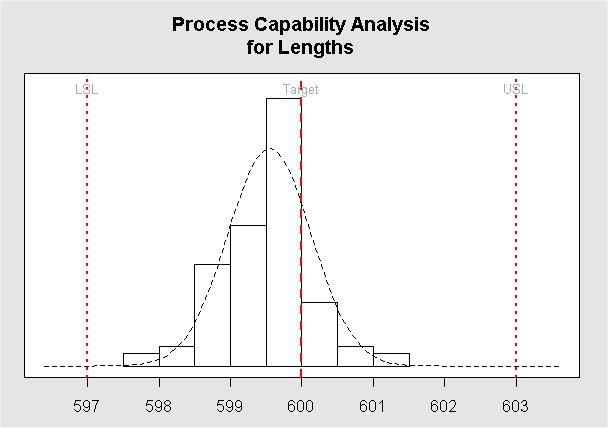
\includegraphics[scale=0.55]{images/ExamQ4hist}
\end{center}
\newpage
%
%Lengths = Values
%
%obj <- qcc(Lengths, type="xbar")
%
%process.capability(obj, spec.limits=c(597,603))



\subsection*{Question 5 Part A (12 Marks)}
% \subsection*{Question 47 - Nelson Rules for Control Charts}
The \textbf{Nelson Rules} are a set of eight decision rules for detecting ``out-of-control" or non-random conditions on control charts. These rules are applied to a control chart on which the magnitude of some variable is plotted against time. The rules are based on the mean value and the standard deviation of the samples.\\

\begin{itemize}
	\item[(i)] ($4 \times 2$ Marks) Discuss any four of these rules, and how they would be used to detect ``out of control" processes. Support your answer with sketch.
\end{itemize}

\bigskip 
\begin{framed}
	\noindent \textit{In your answer, you may make reference to the following properties of the Normal Distribution. Consider the random variable $X$ distributed as
		\[X \sim \mathcal{N}(\mu,\sigma^2)\]
		where $\mu$ is the mean and $\sigma^2$ is the variance of an random variable $X$.}
	\begin{itemize}
		\item $\Pr( \mu - 1\sigma \leq X \leq \mu + 1\sigma ) = 0.6827$
		\item $\Pr( \mu - 2\sigma \leq X \leq \mu + 2\sigma ) = 0.9545$
		\item $\Pr( \mu - 3\sigma \leq X \leq \mu + 3\sigma )= 0.9973$
		
	\end{itemize}
\end{framed}
\newpage



\section*{Formulas and Tables}

\subsection*{Critical Values for Dixon Q Test}


	{
		\Large
		\begin{center}
			\begin{tabular}{|c|c|c|c|}
				\hline  N  & $\alpha=0.10$  & $\alpha=0.05$  & $\alpha=0.01$  \\ \hline
				3  & 0.941 & 0.97  & 0.994 \\ \hline
				4  & 0.765 & 0.829 & 0.926 \\ \hline
				5  & 0.642 & 0.71  & 0.821 \\ \hline
				6  & 0.56  & 0.625 & 0.74  \\ \hline
				7  & 0.507 & 0.568 & 0.68  \\ \hline
				8  & 0.468 & 0.526 & 0.634 \\ \hline
				9  & 0.437 & 0.493 & 0.598 \\ \hline
				10 & 0.412 & 0.466 & 0.568 \\ \hline
				11 & 0.392 & 0.444 & 0.542 \\ \hline
				12 & 0.376 & 0.426 & 0.522 \\ \hline
				13 & 0.361 & 0.41  & 0.503 \\ \hline
				14 & 0.349 & 0.396 & 0.488 \\ \hline
				15 & 0.338 & 0.384 & 0.475 \\ \hline
				16 & 0.329 & 0.374 & 0.463 \\ \hline
			\end{tabular} 
		\end{center}
	}

\subsection*{Two Way ANOVA}
\begin{multicols}{2}
	
\[MS_A = c \times S^2_r\]

\[MS_B = r \times S^2_c\]
\end{multicols}


\subsection*{Control Limits for Control Charts}

\begin{multicols}{2}
	
\[ \bar{\bar{x}} \pm 3\frac{\bar{s}}{c_4\sqrt{n}}\]

\[ \bar{s} \pm 3\frac{c_5\bar{s}}{c_4}\]

\[\left[ \bar{R}D_3, \bar{R}D_4\right]\]
\end{multicols}
\subsection*{$2^3$ Design: Interaction Effects}

\[ AB = \frac{1}{4n} \left[ abc - bc + ab - b - ac + c - a + (1) \right] \]

\[ AC = \frac{1}{4n} \left[ (1) - a + b - ab -c + ac - bc + abc \right] \]

\[ BC = \frac{1}{4n} \left[ (1) + a - b - ab - c - ac + bc + abc \right] \]

\[ABC = \frac{1}{4n} \left[ abc - bc - ac + c - ab + b +  a - (1) \right] \]

\bigskip


\subsection*{Factorial Design: Sums of Squares}

\[\mbox{Effect} =  \frac{\mbox{Contrast}}{4n}\]

\[\mbox{Sums of Squares} =  \frac{\mbox{(Contrast)}^2}{8n}\]

%------------------------------------------------------------------------ %
\normalsize{
\subsection*{Process Capability Indices}
\begin{multicols}{2}
\[ \hat{C}_p = \frac{\mbox{USL} - \mbox{LSL}}{6s}\]

\[ \hat{C}_{pk} = \mbox{min} \left[\frac{\mbox{USL} - \bar{x}}{3s},\frac{\bar{x} - \mbox{LSL}}{3s} \right] \]

\[ \hat{C}_{pm} = \frac{\mbox{USL} - \mbox{LSL}}{6\sqrt{s^2+(\bar{x}-T)^2}}\]
\end{multicols}
	\newpage
	
	%------------------------------------------------------------------------ %
	\Large{
		\subsection*{Factors for Control Charts}
		\begin{tabular}{|c|c|c|c|c|c|c|}
			\hline
			Sample Size (n) 	&	c4 	&	c5 	&	d2 	&	d3 	&	D3 	&	D4	\\	\hline
			2	&	0.7979	&	0.6028	&	1.128	&	0.853	&	0	&	3.267	\\	
			3	&	0.8862	&	0.4633	&	1.693	&	0.888	&	0	&	2.574	\\	
			4	&	0.9213	&	0.3889	&	2.059	&	0.88	&	0	&	2.282	\\	
			5	&	0.9400	&	0.3412	&	2.326	&	0.864	&	0	&	2.114	\\	
			6	&	0.9515	&	0.3076	&	2.534	&	0.848	&	0	&	2.004	\\	
			7	&	0.9594	&	0.282	&	2.704	&	0.833	&	0.076	&	1.924	\\	
			8	&	0.9650	&	0.2622	&	2.847	&	0.82	&	0.136	&	1.864	\\	
			9	&	0.9693	&	0.2459	&	2.970	&	0.808	&	0.184	&	1.816	\\	
			10	&	0.9727	&	0.2321	&	3.078	&	0.797	&	0.223	&	1.777	\\	
			11	&	0.9754	&	0.2204	&	3.173	&	0.787	&	0.256	&	1.744	\\	
			12	&	0.9776	&	0.2105	&	3.258	&	0.778	&	0.283	&	1.717	\\	
			13	&	0.9794	&	0.2019	&	3.336	&	0.770	&	0.307	&	1.693	\\	
			14	&	0.9810	&	0.1940	&	3.407	&	0.763	&	0.328	&	1.672	\\	
			15	&	0.9823	&	0.1873	&	3.472	&	0.756	&	0.347	&	1.653	\\	
			16	&	0.9835	&	0.1809	&	3.532	&	0.750	&	0.363	&	1.637	\\
			17	&	0.9845	&	0.1754	&	3.588	&	0.744	&	0.378	&	1.622	\\
			18	&	0.9854	&	0.1703	&	3.64	&	0.739	&	0.391	&	1.608	\\
			19	&	0.9862	&	0.1656	&	3.689	&	0.734	&	0.403	&	1.597	\\
			20	&	0.9869	&	0.1613	&	3.735	&	0.729	&	0.415	&	1.585	\\
			21	&	0.9876	&	0.1570	&	3.778	&	0.724	&	0.425	&	1.575	\\
			22	&	0.9882	&	0.1532	&	3.819	&	0.720	&	0.434	&	1.566	\\
			23	&	0.9887	&	0.1499	&	3.858	&	0.716	&	0.443	&	1.557	\\
			24	&	0.9892	&	0.1466	&	3.895	&	0.712	&	0.451	&	1.548	\\
			25	&	0.9896	&	0.1438	&	3.931	&	0.708	&	0.459	&	1.541	\\
			\hline
		\end{tabular}
	} % End Large Font
	
\end{document}

Outliers
Boxplots Outliers ( Upper Fence Lower Fence)
Dixon Q-Test
%----------------------------------%
Chi Square 12 Marks
%=====================================================




\end{document}

\newpage
\section{R Code for Part 3}
\begin{verbatim}
ALL <- c(84.32, 84.51, 84.63, 84.61, 84.64, 84.51, 84.62, 84.24, 84.25, 
84.41, 84.13, 84, 84.3, 84.02, 84.29, 84.4, 84.68, 84.28, 84.4, 
84.36, 84.63, 84.14, 84.22, 84.02, 84.48, 84.27, 84.33, 84.22, 
84.5, 83.88, 84.49, 83.91, 84.11, 84.06, 83.99, 84.7, 84.17, 
84.11, 84.36, 84.61, 83.81, 84.15)

\end{verbatim}
%==================================================%
library(xtable)

nu1 <- 2:10
nu2 <- c(5:15,18,21,24,27,30)

L1 <- length(nu1)
L2 <- length(nu2)
CVs <- matrix(ncol=L1,nrow=L2)


for( i in 1:L2){
	for( j in 1:L1){ 
		CVs[i,j] <- round( qf(0.95,i,j),3)
	}
	
}

colnames(CVs)<- nu1

rownames(CVs)<- nu2

xtable(CVs) 

%======================================================================= %
Dixon

chi Square

Normal

One Way ANOVA

Two Way ANOVA interactions

Test Normality

SPC definitions





min=23
max=89
range=65
gap=31
TS =31/65 = 0.47692
CV =0.396 (5\%)
Reject Ho


